\section{View}
The UI will be looking like: \\
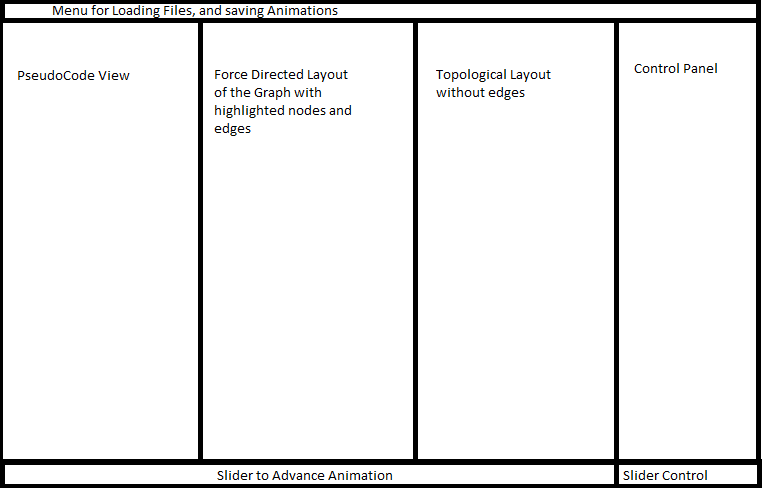
\includegraphics[width=\textwidth]{parts/UIFinished}
\begin{list}{-}{}
\item The left section will be showing the pseudocode of the current active algorithm.
\item The middle sections will show one force directed  graph on the left that will higlight Nodes and the right section will be ordered Topological.

\item Nodes in both graphs will be coloured dynamically.
\begin{list}{-}{}
\item Currently used node will be coloured blue in the left graph.
\item Sources will be colured cyan.
\item Sinks will be colured light gray.
\end{list}
\item Edges will be coloured as following.
\begin{list}{-}{}
\item Active edge will be coloured blue.
\item Reversed edges will be coloured green.
\end{list}
\item The right section will be a Control Panel.
\begin{list}{-}{}
\item for more information see Section Controller

\end{list}
\end{list}



\section{Reason for View}
The reason we use 3 windows for the algorithm is that we needed one representation of the code for the implementation of verbosity, one representation that maps the graph to the code and one representation that maps the reason for the algorythm the topological sorting. By mapping the color in the code with the colors of the 2 window we made a legend without using more space while connecting both windows. The colours are choosen to be easaly recognizable.


